\documentclass[12pt]{article}
\usepackage{verbatim}
\usepackage[dvips]{epsfig}
\usepackage{color}
\usepackage{url}
\usepackage[colorlinks=true]{hyperref}

\begin{document}

\section*{GENESIS: Documentation}

\section*{Installing from a Debian Package}

Debian packages will be available for all major components of GENESIS via sourceforge at:
\begin{itemize}
   \item[]https://sourceforge.net/projects/genesis-sim/
\end{itemize}
\noindent or
\begin{itemize}
   \item[]http://genesis-sim.org/downloads
\end{itemize}
This allows for easy installation via the Debian Package installer GUI.

\subsection*{Installation via Package Installer}

Simply download the desired package so your machine. Go to the directory where it was downloaded. This directory should have an appropriate ``package'' icon.

\begin{figure}[h]
   \centering
   
\includegraphics[scale=0.6
   ]{figures/install-user-deb-icon.eps}
%   \label{fig:df-1}
\end{figure}

Double click on the package icon. A form will appear that gives details about the package such as: Package description, Dependencies, and files to be installed.

\begin{figure}[h]
   \centering
   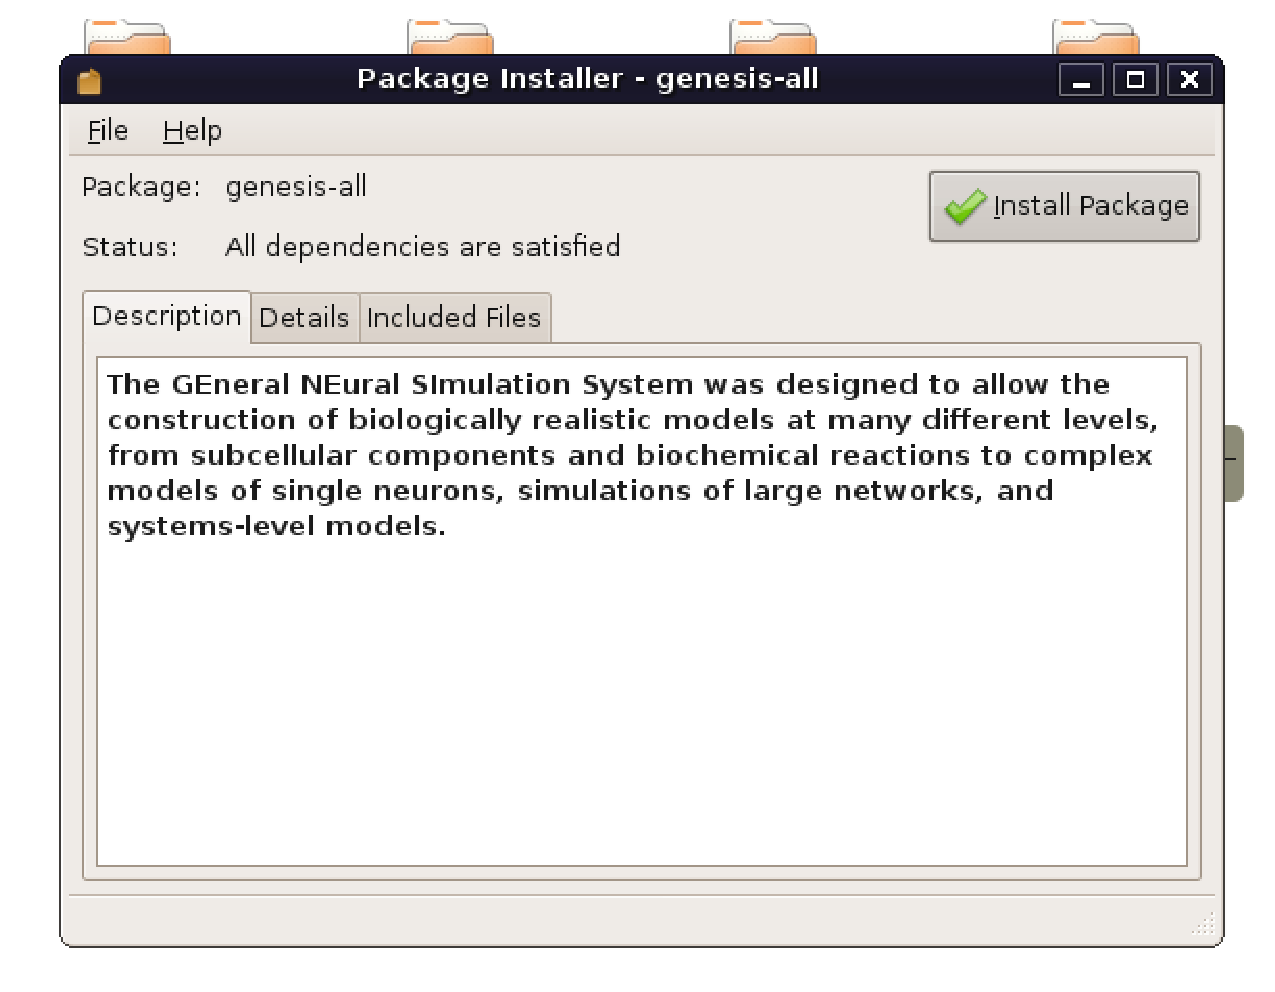
\includegraphics[scale=0.25]{figures/install-user-deb-pkg.eps}
%   \label{fig:df-1}
\end{figure}

\newpage

Click on the Install Package button and you will be prompted to enter in the administrator password for the installation.

\begin{figure}[h]
   \centering
   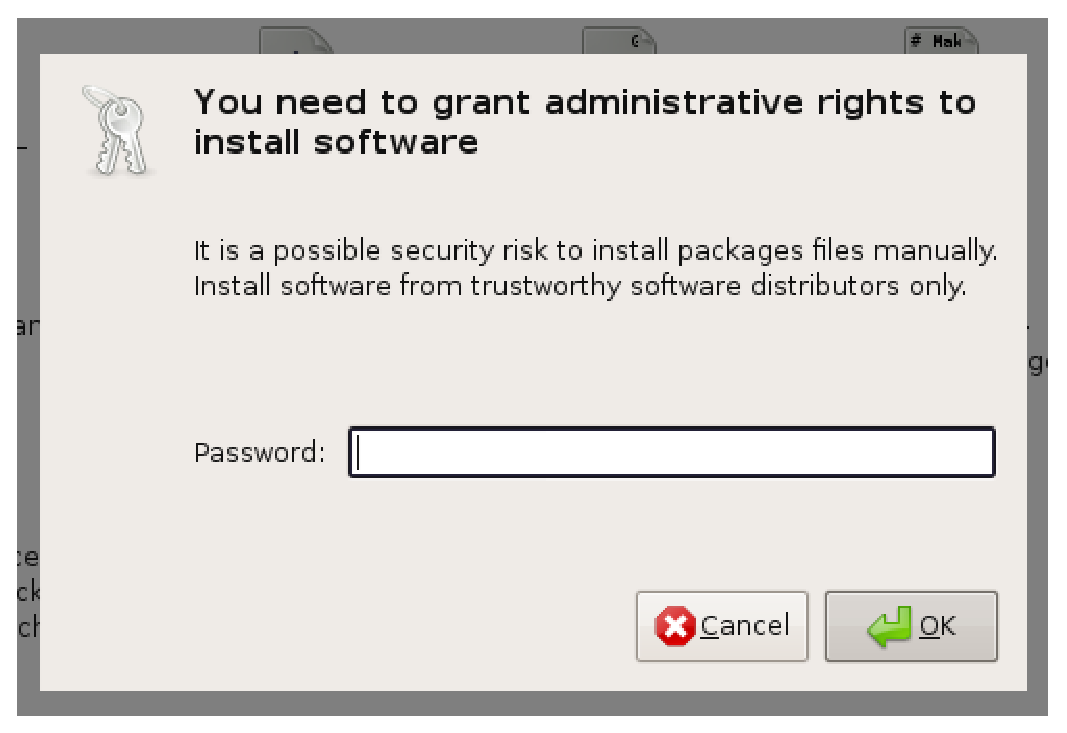
\includegraphics[scale=0.3]{figures/install-user-deb-admin.eps}
%   \label{fig:df-1}
\end{figure}

Once the installation is complete the package installer will prompt with a finished message.

\end{document}
